% Created 2022-09-19 Mon 11:13
\documentclass[9pt, b5paper]{article}
\usepackage{xeCJK}
\usepackage{minted}
\usepackage[T1]{fontenc}
\usepackage[scaled]{beraserif}
\usepackage[scaled]{berasans}
\usepackage[scaled]{beramono}
\usepackage{graphicx}
\usepackage{xcolor}
\usepackage{multirow}
\usepackage{multicol}
\usepackage{float}
\usepackage{textcomp}
\usepackage{algorithm}
\usepackage{algorithmic}
\usepackage{latexsym}
\usepackage{natbib}
\usepackage{geometry}
\geometry{left=1.2cm,right=1.2cm,top=1.5cm,bottom=1.2cm}
\newminted{common-lisp}{fontsize=\footnotesize} 
\usepackage[xetex,colorlinks=true,CJKbookmarks=true,linkcolor=blue,urlcolor=blue,menucolor=blue]{hyperref}
\author{deepwaterooo}
\date{\today}
\title{deepwaterooo deepwateroooMe -- I am the same GitHub account person}
\hypersetup{
  pdfkeywords={},
  pdfsubject={},
  pdfcreator={Emacs 27.1 (Org mode 8.2.7c)}}
\begin{document}

\maketitle
\tableofcontents


\section{Design}
\label{sec-1}
\subsection{MVVM:}
\label{sec-1-1}

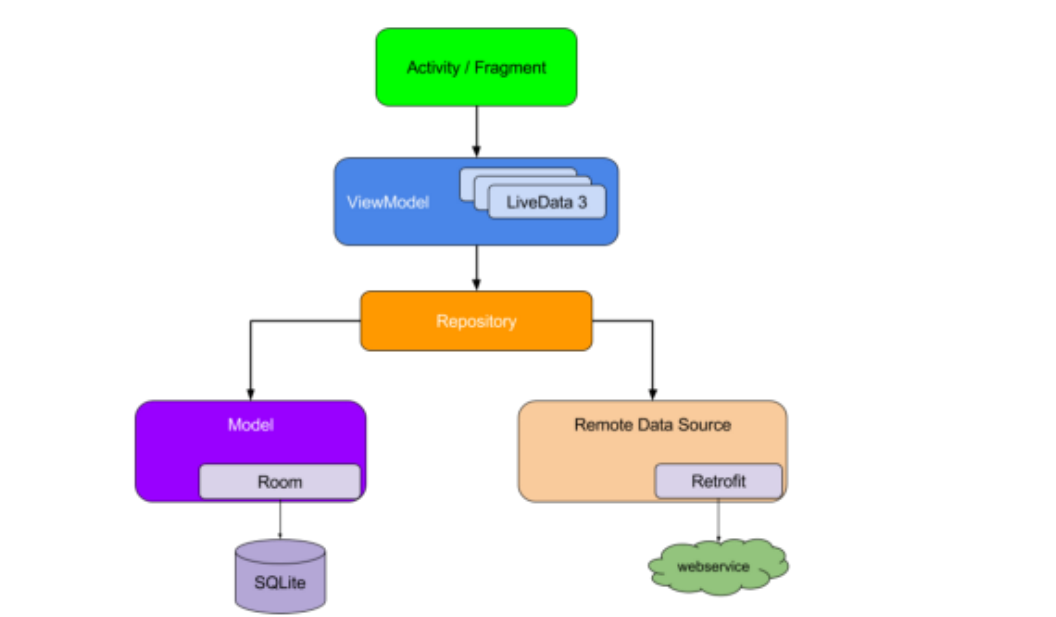
\includegraphics[width=.9\linewidth]{./pic/readme_20220919_110722.png}

\section{Requirement: \url{https://square.github.io/microsite/mobile-interview-project/}}
\label{sec-2}
\begin{itemize}
\item Build an \textbf{employee directory app} that shows a list of employees from the provided endpoint.
\item The app should display a list (or any kind of \textbf{collection view}!) which shows all the employees returned from the JSON endpoint described below.
\item Each item in the view should contain a \textbf{summary of the employee}, including their \textbf{photo, name, and team} at minimum. You may add more information to the summary if you want, or \textbf{sort employees in any fashion} you’d like – sort and group by name, team, etc.
\item There should be some UX to reload the employee list from within the app at any time. The UX can be done in any way you want: \textbf{a button, pull-to-refresh}, etc.
\item If there is any additional UI/UX you would like to add, feel free to do so! We only ask that you please \textbf{do not build any more screens} than this list. Do not worry about building custom controls or UI elements – using \textbf{system-provided, standard elements} is totally fine.
\item Be sure to \textbf{appropriately handle the normal variety of errors when querying an endpoint}. The app should \textbf{display useful loading, empty, and error states} where appropriate. \textbf{If images fail to load, displaying a placeholder} is fine.
\item One extra thing we ask is that you please ensure you \textbf{do not use more network bandwidth than necessary} – \textbf{load expensive resources such as photos on-demand only}.
\item The \textbf{employee list should not be persisted to disk}. You can reload it from the network \textbf{on each app launch and when refresh is requested} — but no more often than that unintentionally.
\item Android developers in particular should take care \textbf{not to make redundant network calls} when the \textbf{phone is rotated, or when memory is low}.
\item \textbf{Images}, however, should \textbf{be cached on disk} so as to not waste device bandwidth. You may use an \textbf{open source image caching solution}, or write your own caching. Do not rely upon HTTP caching for image caching.
\item Note that photos at a given URL will never change. Once one is loaded, you do not need to reload the photo. If an employee’s photo changes, they will be given a new photo URL.
\item \textbf{Tests should be provided for the app}. We do not expect 100\% code coverage, so please use your best judgment for what should be tested. We’re also interested only in \textbf{unit tests}. Feel free to skip snapshot or app tests.
\item If any employee is malformed, it is fine to invalidate the entire list of employees in the response - there is no need to exclude only malformed employees.
\item If there are no employees to show, the app should present an \textbf{empty state} view instead of an empty list.
\end{itemize}

\section{main logs tracked}
\label{sec-3}

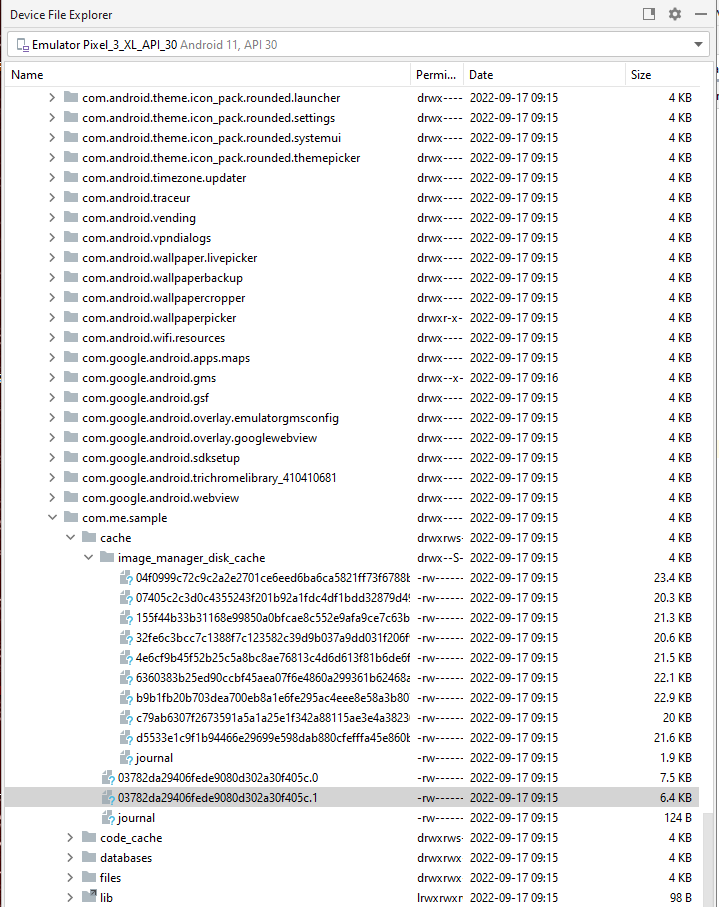
\includegraphics[width=.9\linewidth]{./pic/readme_20220917_093017.png}
\begin{minted}[fontsize=\scriptsize,linenos=false]{ssh}
adb shell am force-stop com.me.sample 

adb shell am kill com.me.sample 
adb shell ==> ps -A | grep com.me.sample # 前后对比就能够验证出,它是真死了

adb shell am kill-all              
\end{minted}
\begin{minted}[fontsize=\scriptsize,linenos=false]{text}
com.me.sample D/MainActivity: onCreate() 
com.me.sample I/ViewRootImpl@9fdb9bb[MainActivity]: setView = com.android.internal.policy.DecorView@ec3fbc TM=true
com.me.sample D/MainActivity: onStart() 
com.me.sample I/ViewRootImpl@9fdb9bb[MainActivity]: stopped(false) old=false
com.me.sample D/MainActivity: onResume() 
com.me.sample I/ViewRootImpl@e7eb0db[MainActivity]: setView = com.android.internal.policy.DecorView@798929f TM=true
com.me.sample I/ViewRootImpl@9fdb9bb[MainActivity]: Relayout returned: old=(0,142,1440,2872) new=(510,1297,930,1717) req=(420,420)0 dur=5 res=0x7 s={true -5476376617398110128} ch=true fn=-1
com.me.sample I/ViewRootImpl@9fdb9bb[MainActivity]: [DP] dp(1) 1 android.view.ViewRootImpl.reportNextDraw:11374 android.view.ViewRootImpl.performTraversals:4167 android.view.ViewRootImpl.doTraversal:2893 
com.me.sample I/BufferQueueProducer: [ViewRootImpl@9fdb9bb[MainActivity]#0(BLAST Consumer)0](id:297f00000000,api:1,p:10623,c:10623) queueBuffer: queued for the first time.
com.me.sample I/ViewRootImpl@e7eb0db[MainActivity]: Relayout returned: old=(0,0,1440,3040) new=(0,0,1440,3040) req=(1440,3040)0 dur=5 res=0x7 s={true -5476376617397988048} ch=true fn=-1
com.me.sample I/ViewRootImpl@e7eb0db[MainActivity]: [DP] dp(1) 1 android.view.ViewRootImpl.reportNextDraw:11374 android.view.ViewRootImpl.performTraversals:4167 android.view.ViewRootImpl.doTraversal:2893 
com.me.sample I/BufferQueueProducer: [ViewRootImpl@e7eb0db[MainActivity]#1(BLAST Consumer)1](id:297f00000001,api:1,p:10623,c:10623) queueBuffer: queued for the first time.
com.me.sample I/ViewRootImpl@e7eb0db[MainActivity]: [DP] pdf(0) 1 android.view.ViewRootImpl.lambda$addFrameCompleteCallbackIfNeeded$3$ViewRootImpl:4969 android.view.ViewRootImpl$$ExternalSyntheticLambda16.run:6 android.os.Hander.handleCallback:938 
com.me.sample I/ViewRootImpl@e7eb0db[MainActivity]: [DP] rdf()
com.me.sample D/ViewRootImpl@e7eb0db[MainActivity]: reportDrawFinished (fn: -1) 
com.me.sample I/ViewRootImpl@9fdb9bb[MainActivity]: [DP] pdf(0) 1 android.view.ViewRootImpl.lambda$addFrameCompleteCallbackIfNeeded$3$ViewRootImpl:4969 android.view.ViewRootImpl$$ExternalSyntheticLambda16.run:6 android.os.Handler.handleCallback:938 
com.me.sample I/ViewRootImpl@9fdb9bb[MainActivity]: [DP] rdf()
com.me.sample D/ViewRootImpl@9fdb9bb[MainActivity]: reportDrawFinished (fn: -1) 
com.me.sample I/ViewRootImpl@9fdb9bb[MainActivity]: dispatchDetachedFromWindow
com.me.sample I/ViewRootImpl@e7eb0db[MainActivity]: MSG_WINDOW_FOCUS_CHANGED 1 1
com.me.sample I/MainActivity: Started in onCreate(), running until onDestory(): 0
com.me.sample I/MainActivity: Started in onCreate(), running until onDestory(): 1
com.me.sample I/MainActivity: Started in onCreate(), running until onDestory(): 2

com.me.sample D/MainActivity: onCreate() 
com.me.sample I/ViewRootImpl@cfdc231[MainActivity]: setView = com.android.internal.policy.DecorView@11ea6c1 TM=true
com.me.sample D/MainActivity: onStart() 
com.me.sample I/ViewRootImpl@cfdc231[MainActivity]: stopped(false) old=false
com.me.sample D/MainActivity: onResume() 
com.me.sample I/ViewRootImpl@ccc5e51[MainActivity]: setView = com.android.internal.policy.DecorView@41dfb5 TM=true
com.me.sample I/ViewRootImpl@cfdc231[MainActivity]: Resizing android.view.ViewRootImpl@d4d842: frame=[510,1297][930,1717] reportDraw=true forceLayout=false backDropFrame=Rect(0, 0 - 420, 420)
com.me.sample I/ViewRootImpl@cfdc231[MainActivity]: Relayout returned: old=(0,142,1440,2872) new=(510,1297,930,1717) req=(420,420)0 dur=6 res=0x7 s={true -5476376617398049088} ch=true fn=-1
com.me.sample I/ViewRootImpl@cfdc231[MainActivity]: [DP] dp(1) 1 android.view.ViewRootImpl.reportNextDraw:11374 android.view.ViewRootImpl.performTraversals:4167 android.view.ViewRootImpl.doTraversal:2893 
com.me.sample I/BufferQueueProducer: [ViewRootImpl@cfdc231[MainActivity]#0(BLAST Consumer)0](id:2e8c00000000,api:1,p:11916,c:11916) queueBuffer: queued for the first time.
com.me.sample I/ViewRootImpl@ccc5e51[MainActivity]: Relayout returned: old=(0,0,1440,3040) new=(0,0,1440,3040) req=(1440,3040)0 dur=6 res=0x7 s={true -5476376617398005488} ch=true fn=-1
com.me.sample I/ViewRootImpl@ccc5e51[MainActivity]: [DP] dp(1) 1 android.view.ViewRootImpl.reportNextDraw:11374 android.view.ViewRootImpl.performTraversals:4167 android.view.ViewRootImpl.doTraversal:2893 
com.me.sample I/BufferQueueProducer: [ViewRootImpl@ccc5e51[MainActivity]#1(BLAST Consumer)1](id:2e8c00000001,api:1,p:11916,c:11916) queueBuffer: queued for the first time.
com.me.sample I/ViewRootImpl@ccc5e51[MainActivity]: [DP] pdf(0) 1 android.view.ViewRootImpl.lambda$addFrameCompleteCallbackIfNeeded$3$ViewRootImpl:4969 android.view.ViewRootImpl$$ExternalSyntheticLambda16.run:6 android.os.Handler.handleCallback:938 
com.me.sample I/ViewRootImpl@ccc5e51[MainActivity]: [DP] rdf()
com.me.sample D/ViewRootImpl@ccc5e51[MainActivity]: reportDrawFinished (fn: -1) 
com.me.sample I/ViewRootImpl@cfdc231[MainActivity]: [DP] pdf(0) 1 android.view.ViewRootImpl.lambda$addFrameCompleteCallbackIfNeeded$3$ViewRootImpl:4969 android.view.ViewRootImpl$$ExternalSyntheticLambda16.run:6 android.os.Handler.handleCallback:938 
com.me.sample I/ViewRootImpl@cfdc231[MainActivity]: [DP] rdf()
com.me.sample D/ViewRootImpl@cfdc231[MainActivity]: reportDrawFinished (fn: -1) 
com.me.sample I/ViewRootImpl@cfdc231[MainActivity]: handleResized, msg = 5 frames=ClientWindowFrames{frame=[510,1297][930,1717] display=[0,142][1440,2872] backdrop=[0,0][420,420]} forceNextWindowRelayout=false displayId=0 frameChanged=false backdropFrameChanged=true configChanged=false displayChanged=false mNextDrawUseBlastSync=false mergedConfiguration={mGlobalConfig={1.1 311mcc480mnc [en_US] ldltr sw411dp w411dp h780dp 560dpi nrml long hdr widecg port finger -keyb/v/h -nav/h winConfig={ mBounds=Rect(0, 0 - 1440, 3040) mAppBounds=Rect(0, 142 - 1440, 2872) mMaxBounds=Rect(0, 0 - 1440, 3040) mWindowingMode=fullscreen mDisplayWindowingMode=fullscreen mActivityType=undefined mAlwaysOnTop=undefined mRotation=ROTATION_0 mPopOver=off mFreeformTaskPinningState=unpinned} s.26854 fontWeightAdjustment=0 ff=0 bf=0 bts=0 desktop/d dm/n dc/d ?dcui ?dcaf enb/d themeSeq=0} mOverrideConfig={1.1 311mcc480mnc [en_US] ldltr sw411dp w411dp h780dp 560dpi nrml long hdr widecg port finger -keyb/v/h -nav/h winConfig={ mBounds=Rect(0, 0 - 1440, 3040) mAppBounds=Rect(0, 142 - 1440, 2872) mMaxBounds=Rect(0, 0 - 1440, 3040) mWindowingMode=fullscreen mDisplayWindowingMode=fullscreen mActivityType=standard mAlwaysOnTop=undefined mRotation=ROTATION_0 mPopOver=off mFreeformTaskPinningState=unpinned} s.1 fontWeightAdjustment=0 ff=0 bf=0 bts=0 desktop/d dm/n dc/d ?dcui ?dcaf enb/d themeSeq=0}}
com.me.sample I/ViewRootImpl@cfdc231[MainActivity]: [DP] dp(1) 1 android.view.ViewRootImpl.reportNextDraw:11374 android.view.ViewRootImpl.handleResized:2204 android.view.ViewRootImpl.access$1200:294
\end{minted}
\begin{itemize}
\item Click and select the app from the recently used app list, and relanuching process without requesting data through http requests:
\end{itemize}
\begin{minted}[fontsize=\scriptsize,linenos=false]{text}
com.me.sample D/MainActivity: onCreate() 
com.me.sample I/ViewRootImpl@1413ed8[MainActivity]: setView = com.android.internal.policy.DecorView@11529a TM=true
com.me.sample D/MainActivity: onStart() 
com.me.sample D/MainActivity: onRestoreInstanceState() 
com.me.sample I/ViewRootImpl@1413ed8[MainActivity]: stopped(false) old=false
com.me.sample D/MainActivity: onResume() 
com.me.sample I/ViewRootImpl@a363778[MainActivity]: setView = com.android.internal.policy.DecorView@e9d0fec TM=true
com.me.sample I/ViewRootImpl@1413ed8[MainActivity]: Relayout returned: old=(0,142,1440,2872) new=(510,1297,930,1717) req=(420,420)0 dur=5 res=0x7 s={true -5476376617398040368} ch=true fn=-1
com.me.sample I/ViewRootImpl@1413ed8[MainActivity]: [DP] dp(1) 1 android.view.ViewRootImpl.reportNextDraw:11374 android.view.ViewRootImpl.performTraversals:4167 android.view.ViewRootImpl.doTraversal:2893 
com.me.sample I/BufferQueueProducer: [ViewRootImpl@1413ed8[MainActivity]#0(BLAST Consumer)0](id:610c00000000,api:1,p:24844,c:24844) queueBuffer: queued for the first time.
com.me.sample I/ViewRootImpl@a363778[MainActivity]: Relayout returned: old=(0,0,1440,3040) new=(0,0,1440,3040) req=(1440,3040)0 dur=4 res=0x7 s={true -5476376617398005488} ch=true fn=-1
com.me.sample I/ViewRootImpl@a363778[MainActivity]: [DP] dp(1) 1 android.view.ViewRootImpl.reportNextDraw:11374 android.view.ViewRootImpl.performTraversals:4167 android.view.ViewRootImpl.doTraversal:2893 
com.me.sample I/BufferQueueProducer: [ViewRootImpl@a363778[MainActivity]#1(BLAST Consumer)1](id:610c00000001,api:1,p:24844,c:24844) queueBuffer: queued for the first time.
com.me.sample I/ViewRootImpl@a363778[MainActivity]: [DP] pdf(0) 1 android.view.ViewRootImpl.lambda$addFrameCompleteCallbackIfNeeded$3$ViewRootImpl:4969 android.view.ViewRootImpl$$ExternalSyntheticLambda16.run:6 android.os.Handler.handleCallback:938 
com.me.sample I/ViewRootImpl@a363778[MainActivity]: [DP] rdf()
com.me.sample D/ViewRootImpl@a363778[MainActivity]: reportDrawFinished (fn: -1) 
com.me.sample I/ViewRootImpl@1413ed8[MainActivity]: [DP] pdf(0) 1 android.view.ViewRootImpl.lambda$addFrameCompleteCallbackIfNeeded$3$ViewRootImpl:4969 android.view.ViewRootImpl$$ExternalSyntheticLambda16.run:6 android.os.Handler.handleCallback:938 
com.me.sample I/ViewRootImpl@1413ed8[MainActivity]: [DP] rdf()
com.me.sample D/ViewRootImpl@1413ed8[MainActivity]: reportDrawFinished (fn: -1) 
com.me.sample I/ViewRootImpl@1413ed8[MainActivity]: dispatchDetachedFromWindow
com.me.sample I/ViewRootImpl@a363778[MainActivity]: MSG_WINDOW_FOCUS_CHANGED 1 1
\end{minted}

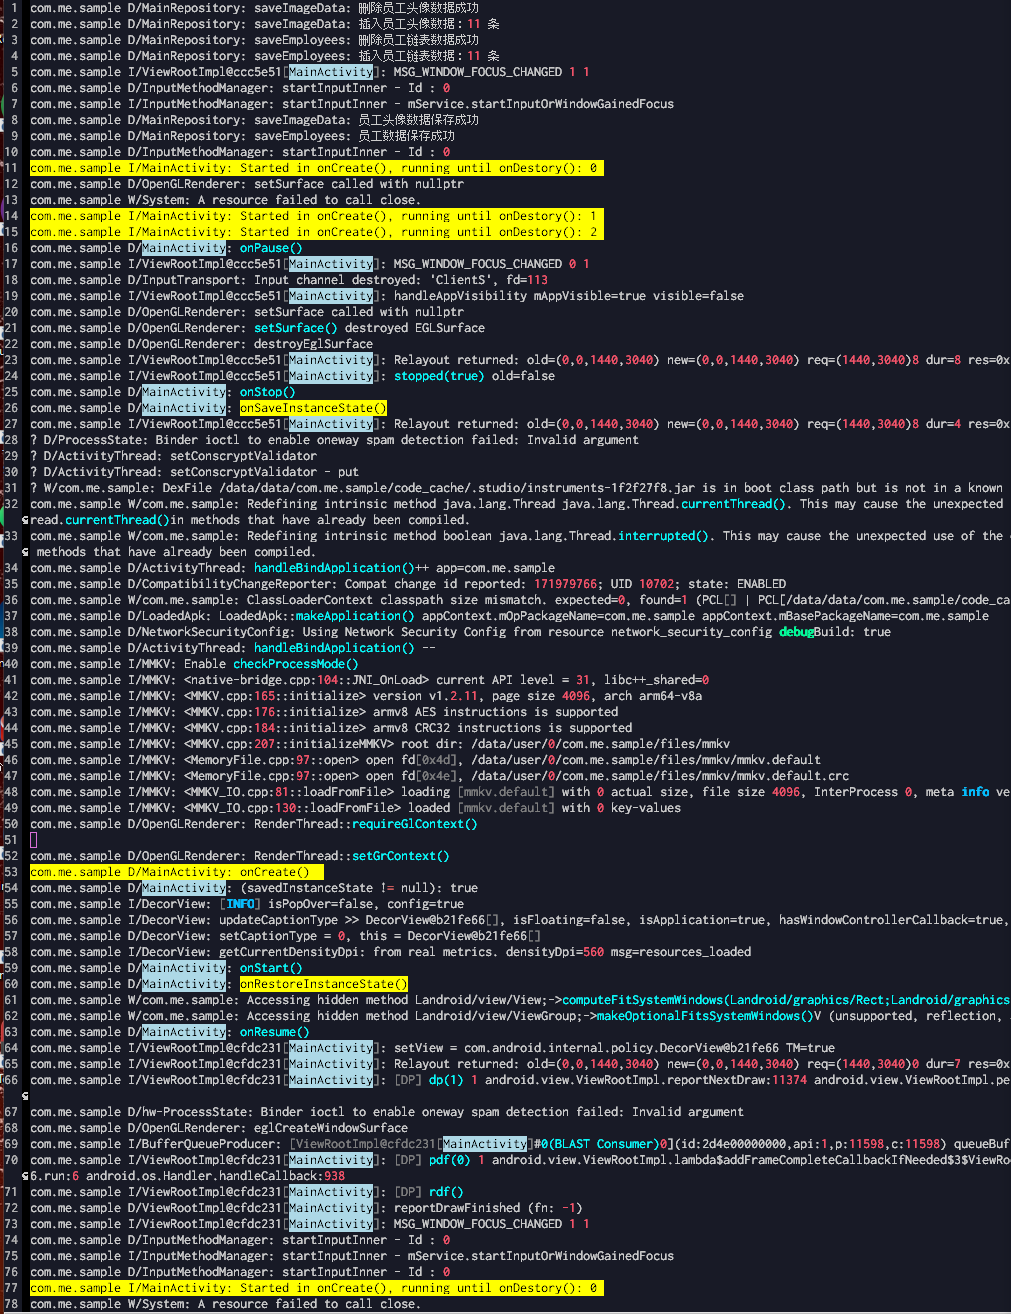
\includegraphics[width=.9\linewidth]{./pic/readme_20220915_225835.png}
\begin{minted}[fontsize=\scriptsize,linenos=false]{text}
com.me.sample D/MainRepository: saveImageData: 删除员工头像数据成功
com.me.sample D/MainRepository: saveImageData: 插入员工头像数据:11条
com.me.sample D/MainRepository: saveEmployees: 删除员工链表数据成功
com.me.sample D/MainRepository: saveEmployees: 插入员工链表数据:11条
com.me.sample I/ViewRootImpl@ccc5e51[MainActivity]: MSG_WINDOW_FOCUS_CHANGED 1 1
com.me.sample D/InputMethodManager: startInputInner - Id : 0
com.me.sample I/InputMethodManager: startInputInner - mService.startInputOrWindowGainedFocus
com.me.sample D/MainRepository: saveImageData: 员工头像数据保存成功
com.me.sample D/MainRepository: saveEmployees: 员工数据保存成功
com.me.sample D/InputMethodManager: startInputInner - Id : 0
com.me.sample I/MainActivity: Started in onCreate(), running until onDestory(): 0
com.me.sample D/OpenGLRenderer: setSurface called with nullptr
com.me.sample W/System: A resource failed to call close. 
com.me.sample I/MainActivity: Started in onCreate(), running until onDestory(): 1
com.me.sample I/MainActivity: Started in onCreate(), running until onDestory(): 2
com.me.sample D/MainActivity: onPause() 
com.me.sample I/ViewRootImpl@ccc5e51[MainActivity]: MSG_WINDOW_FOCUS_CHANGED 0 1
com.me.sample D/InputTransport: Input channel destroyed: 'ClientS', fd=113
com.me.sample I/ViewRootImpl@ccc5e51[MainActivity]: handleAppVisibility mAppVisible=true visible=false
com.me.sample D/OpenGLRenderer: setSurface called with nullptr
com.me.sample D/OpenGLRenderer: setSurface() destroyed EGLSurface
com.me.sample D/OpenGLRenderer: destroyEglSurface
com.me.sample I/ViewRootImpl@ccc5e51[MainActivity]: Relayout returned: old=(0,0,1440,3040) new=(0,0,1440,3040) req=(1440,3040)8 dur=8 res=0x5 s={false 0} ch=true fn=7
com.me.sample I/ViewRootImpl@ccc5e51[MainActivity]: stopped(true) old=false
com.me.sample D/MainActivity: onStop() 
com.me.sample D/MainActivity: onSaveInstanceState()
com.me.sample I/ViewRootImpl@ccc5e51[MainActivity]: Relayout returned: old=(0,0,1440,3040) new=(0,0,1440,3040) req=(1440,3040)8 dur=4 res=0x5 s={false 0} ch=false fn=-1
? I/com.me.sample: Late-enabling -Xcheck:jni
? E/USNET: USNET: appName: com.me.sample
? D/ProcessState: Binder ioctl to enable oneway spam detection failed: Invalid argument
? D/ActivityThread: setConscryptValidator
? D/ActivityThread: setConscryptValidator - put
? W/com.me.sample: DexFile /data/data/com.me.sample/code_cache/.studio/instruments-1f2f27f8.jar is in boot class path but is not in a known location
com.me.sample W/com.me.sample: Redefining intrinsic method java.lang.Thread java.lang.Thread.currentThread(). This may cause the unexpected use of the original definition of java.lang.Thread java.lang.Thread.currentThread()in methods that have already been compiled.
com.me.sample W/com.me.sample: Redefining intrinsic method boolean java.lang.Thread.interrupted(). This may cause the unexpected use of the original definition of boolean java.lang.Thread.interrupted()in methods that have already been compiled.
com.me.sample D/ActivityThread: handleBindApplication()++ app=com.me.sample
com.me.sample D/CompatibilityChangeReporter: Compat change id reported: 171979766; UID 10702; state: ENABLED
com.me.sample W/com.me.sample: ClassLoaderContext classpath size mismatch. expected=0, found=1 (PCL[] | PCL[/data/data/com.me.sample/code_cache/.overlay/base.apk/classes14.dex*1294054685])
com.me.sample D/LoadedApk: LoadedApk::makeApplication() appContext.mOpPackageName=com.me.sample appContext.mBasePackageName=com.me.sample
com.me.sample D/NetworkSecurityConfig: Using Network Security Config from resource network_security_config debugBuild: true
com.me.sample D/ActivityThread: handleBindApplication() --
com.me.sample I/MMKV: Enable checkProcessMode()
com.me.sample I/MMKV: <native-bridge.cpp:104::JNI_OnLoad> current API level = 31, libc++_shared=0
com.me.sample I/MMKV: <MMKV.cpp:165::initialize> version v1.2.11, page size 4096, arch arm64-v8a
com.me.sample I/MMKV: <MMKV.cpp:176::initialize> armv8 AES instructions is supported
com.me.sample I/MMKV: <MMKV.cpp:184::initialize> armv8 CRC32 instructions is supported
com.me.sample I/MMKV: <MMKV.cpp:207::initializeMMKV> root dir: /data/user/0/com.me.sample/files/mmkv
com.me.sample I/MMKV: <MemoryFile.cpp:97::open> open fd[0x4d], /data/user/0/com.me.sample/files/mmkv/mmkv.default
com.me.sample I/MMKV: <MemoryFile.cpp:97::open> open fd[0x4e], /data/user/0/com.me.sample/files/mmkv/mmkv.default.crc
com.me.sample I/MMKV: <MMKV_IO.cpp:81::loadFromFile> loading [mmkv.default] with 0 actual size, file size 4096, InterProcess 0, meta info version:1
com.me.sample I/MMKV: <MMKV_IO.cpp:130::loadFromFile> loaded [mmkv.default] with 0 key-values
com.me.sample D/OpenGLRenderer: RenderThread::requireGlContext()

com.me.sample D/OpenGLRenderer: RenderThread::setGrContext()
com.me.sample D/MainActivity: onCreate() 
com.me.sample D/MainActivity: (savedInstanceState != null): true
com.me.sample I/DecorView: [INFO] isPopOver=false, config=true
com.me.sample I/DecorView: updateCaptionType >> DecorView@b21fe66[], isFloating=false, isApplication=true, hasWindowControllerCallback=true, hasWindowDecorCaption=false
com.me.sample D/DecorView: setCaptionType = 0, this = DecorView@b21fe66[]
com.me.sample I/DecorView: getCurrentDensityDpi: from real metrics. densityDpi=560 msg=resources_loaded
com.me.sample D/MainActivity: onStart() 
com.me.sample D/MainActivity: onRestoreInstanceState() 
com.me.sample W/com.me.sample: Accessing hidden method Landroid/view/View;->computeFitSystemWindows(Landroid/graphics/Rect;Landroid/graphics/Rect;)Z (unsupported, reflection, allowed)
com.me.sample W/com.me.sample: Accessing hidden method Landroid/view/ViewGroup;->makeOptionalFitsSystemWindows()V (unsupported, reflection, allowed)
com.me.sample D/MainActivity: onResume() 
com.me.sample I/ViewRootImpl@cfdc231[MainActivity]: setView = com.android.internal.policy.DecorView@b21fe66 TM=true
com.me.sample I/ViewRootImpl@cfdc231[MainActivity]: Relayout returned: old=(0,0,1440,3040) new=(0,0,1440,3040) req=(1440,3040)0 dur=7 res=0x7 s={true -5476376617398057808} ch=true fn=-1
com.me.sample I/ViewRootImpl@cfdc231[MainActivity]: [DP] dp(1) 1 android.view.ViewRootImpl.reportNextDraw:11374 android.view.ViewRootImpl.performTraversals:4167 android.view.ViewRootImpl.doTraversal:2893 
com.me.sample D/hw-ProcessState: Binder ioctl to enable oneway spam detection failed: Invalid argument
com.me.sample D/OpenGLRenderer: eglCreateWindowSurface
com.me.sample I/BufferQueueProducer: [ViewRootImpl@cfdc231[MainActivity]#0(BLAST Consumer)0](id:2d4e00000000,api:1,p:11598,c:11598) queueBuffer: queued for the first time.
com.me.sample I/ViewRootImpl@cfdc231[MainActivity]: [DP] pdf(0) 1 android.view.ViewRootImpl.lambda$addFrameCompleteCallbackIfNeeded$3$ViewRootImpl:4969 android.view.ViewRootImpl$$ExternalSyntheticLambda16.run:6 android.os.Handler.handleCallback:938 
com.me.sample I/ViewRootImpl@cfdc231[MainActivity]: [DP] rdf()
com.me.sample D/ViewRootImpl@cfdc231[MainActivity]: reportDrawFinished (fn: -1) 
com.me.sample I/ViewRootImpl@cfdc231[MainActivity]: MSG_WINDOW_FOCUS_CHANGED 1 1
com.me.sample D/InputMethodManager: startInputInner - Id : 0
com.me.sample I/InputMethodManager: startInputInner - mService.startInputOrWindowGainedFocus
com.me.sample D/InputMethodManager: startInputInner - Id : 0
com.me.sample I/MainActivity: Started in onCreate(), running until onDestory(): 0
com.me.sample W/System: A resource failed to call close.
\end{minted}
\begin{itemize}
\item \url{https://www.jianshu.com/p/8311410de676})
\item \url{https://blog.csdn.net/fitaotao/article/details/117519733}
\item \url{https://github.com/xitu/gold-miner/blob/master/TODO/getting-started-with-retrofit.md}
\item \url{https://developer.aliyun.com/article/609862}
\end{itemize}
% Emacs 27.1 (Org mode 8.2.7c)
\end{document}